\section{Methodology}

Thus, we hypothesize that the key to increasing model robustness lies in the construction and augmentation of a synthetic dataset. In-silico construction immediately solves two major problems with NIDS datasets: it is, by design, fully documented and reproducible, as the dataset no longer consists of the actual PCAP files: it is the descriptions of the network and the attacks that form the dataset. Datasets constructed in this way can also be easily extended with new classes of attacks, variants of existing classes of attacks, and new network configurations. 

The previously mentioned ConCap framework \cite{concap}, built on Kubernetes and Docker, has been proposed for the synthetic dataset construction that we describe above. We use ConCap to verify our hypothesis and employ the following methodology: in Section \ref{cic_analysis}, we analyse the CIC-IDS-2017 and the literature surrounding it in depth. In Section \ref{reconstruction}, we describe the reconstruction process and any significant choices we make. Then finally, in Section \ref{experiments}, we describe our testing methodology to prove or disprove the hypothesis.

\subsection{Analysis of CIC-IDS-2017}\label{cic_analysis}
CIC-IDS-2017 dataset has been constructed by the Canadian Institute for Cybersecurity in 2017 to address the then-prevalent issues with existing NIDS datasets. Dataset authors focus on generating realistic background traffic, in addition to seven attack classes: Bruteforce, Denial-of-Service, Heartbleed, Web Attack infiltration, Botnet, Distributed-Denial-of-Service and Portscanning. The dataset consists of traffic captures as PCAP files during the work week of July 3, 2017. 

The dataset contains a relatively simple victim network (compared to its larger cousin, CIC-IDS-2018), consisting of a Windows Server, a Ubuntu 16 webserver and a Ubuntu 12 server, as well as two Ubuntu 14.04, two Ubuntu 16.04, a Windows 7, Windows 8.1-64, Windows Vista, Windows 10 Pro and a Macintosh computers, nice in total. The attacker network consists of one Kali Linux and three Windows 8.1 machines. The attackers communicate with the victim network over the internet, appearing in the PCAP files under the IP address \texttt{172.16.0.1}. There is further network infrastructure present, but it is inconsequential for our purposes. Figure \ref{fig:cic_2017_testbed} \cite{cic_2017} shows a schematic of the testbed.

Most attacks (Bruteforce, DoS, Web Attacks, DDoS, Portscan) are conducted against a single host, the Ubuntu 16.04 webserver. We reconstruct this webserver as faithfully as possible, basing ourselves on the services revealed by the Portscan attack on Friday.

\begin{figure}
	\centering
	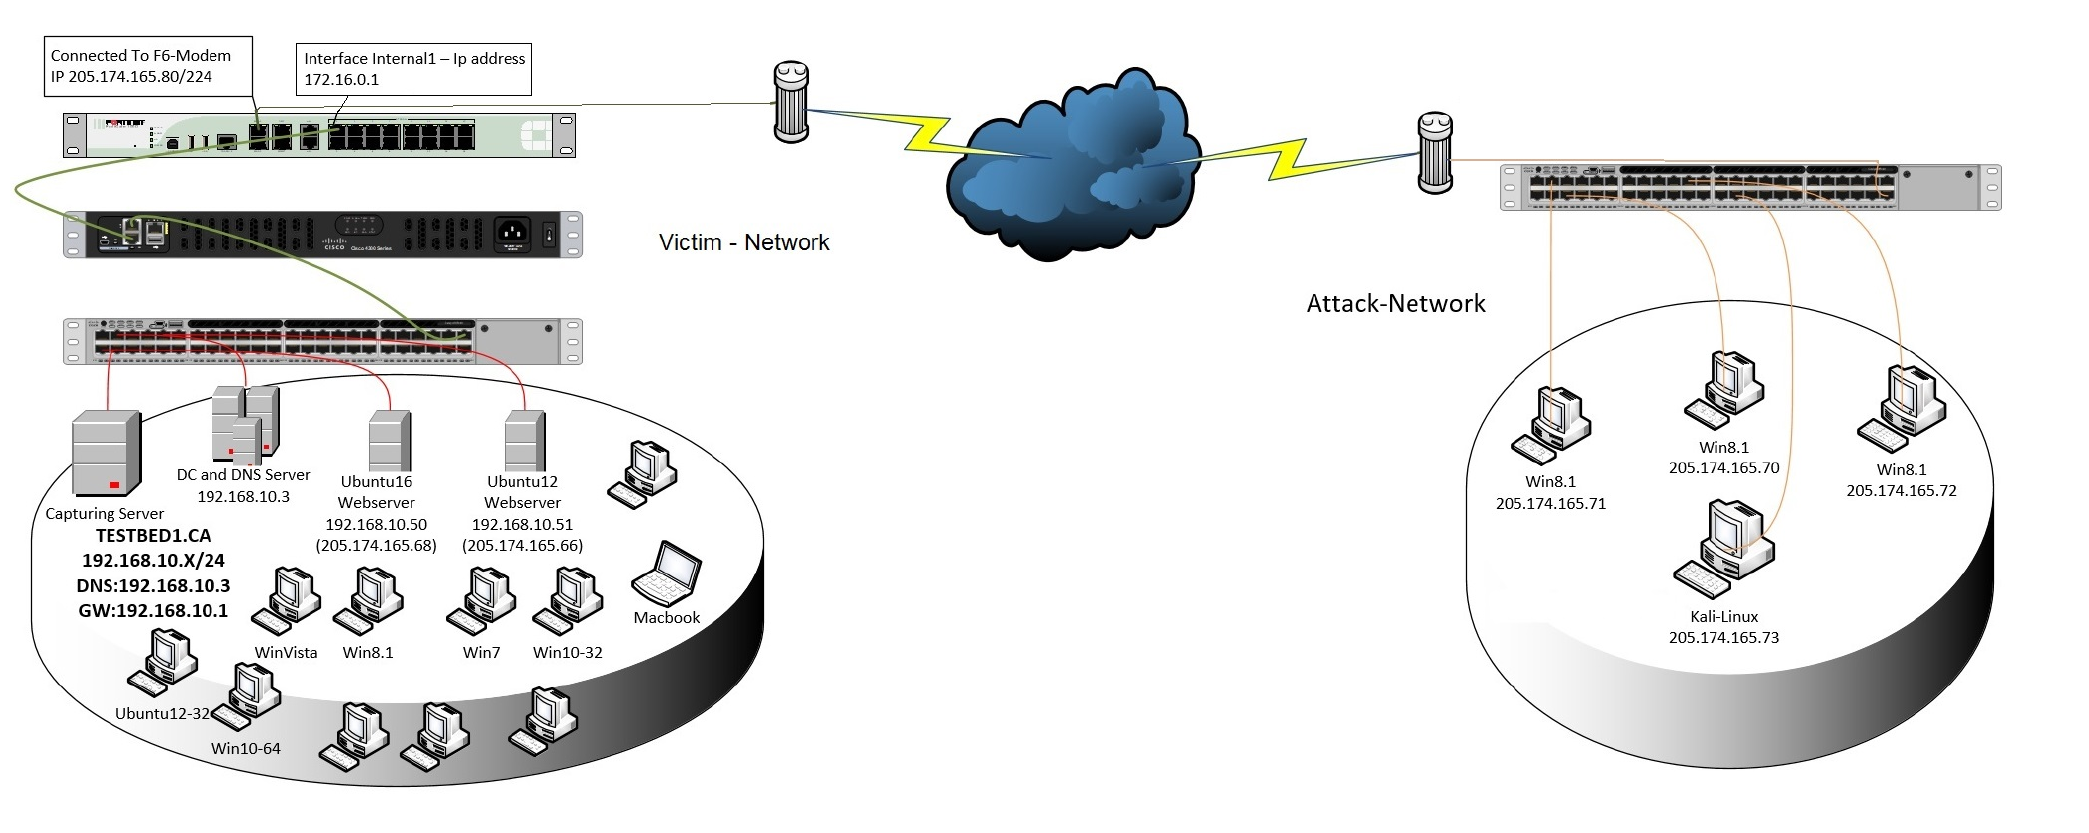
\includegraphics[width=0.9\linewidth]{screenshot001}
	\caption{Architecture of CIC-IDS-2017 testbed}
	\label{fig:cic_2017_testbed}
\end{figure}



\subsubsection{Monday}

On Monday, no attacks take place, only background traffic is happening. The authors utilise a B-Profile system \cite{b_profile} for benign traffic generation "to profile abstract behavior of human interactions and generates naturalistic background traffic"\cite{cic_2017}. The traffic capture of this day consists of "abstract behaviour of 25 users based on the HTTP, HTTPS, FTP, SSH, and email protocols." \cite{cic_2017} and provides an excellent source of benign samples that we later use to balance the training sets.

\subsubsection{Tuesday}
On Tuesday, in addition to the background traffic as seen on Monday, we see the first attack class take place: Bruteforce. In the morning, an FTP Bruteforce attack is performed using Patator \cite{patator}. This attack is run against the iscxtap user, with various passwords being tried from an unknown wordlist. In the afternoon, SSH Bruteforce attack is performed using presumably the same tool. Due to inherent encryption of SSH traffic, it is unclear against which user the attack is conducted or what wordlist is used for passwords.

\subsubsection{Wednesday}
On Wednesday, Denial-of-Service (DoS) attacks are launched against the Ubuntu 16 webserver. The dataset consists of four DoS attacks conducted with the tools Slowhttptest \cite{slowhttptest}, GoldenEye \cite{goldeneye} and HULK \cite{hulk}. In the afternoon, the vulnerable OpenSSH server falls victim to the Heartbleed bug \cite{heartbleed} exploitation.  

Slowhttptest attacks the server by heavily fragmenting the HTTP request body into small chunks and slowly sending them to the server. By slowly receiving the chunks, the server is forced to maintain the connection and waste resources. As the server is limited in how many requests it can serve at any given time, a denial of service occurs.

Slowloris works similarly to Slowhttptest, but instead of fragmenting the body, the Headers section of the HTTP request is fragmented. These fragmented headers are then slowly sent to the server, again forcing it to keep the connection alive and prevent legitimate requests from being processed.

GoldenEye abuses the HTTP \texttt{Connection} and \texttt{Cache-Control} headers to maintain the open connection. Through the Connection HTTP header, the server can be instructed to keep the connection alive (through the \texttt{keep-alive} option) to allow additional requests to take place over the same connection. Cache-Control header contains instructions for the browser and shared caches. By setting this header to \texttt{no-cache,max-age=0}, it effectively disables connection busting through caches.
GoldenEye abuses these headers by opening a large number of connections, effectively exhausting the connection pool of the server, and denying service to legitimate clients.

Http Unbearable Load King (HULK) attacks the server by flooding it with raw UDP packets. As UDP does not require a three-way handshake to set up a connection like TCP does, this attack can simply flood the server with packets it needs to handle, overloading it. HULK works best as a distributed attack with multiple malicious clients flooding the target. However, this attack is also easy to stop through a proper firewall configuration. 

The Heartbleed bug \cite{heartbleed} was first discovered in 2014 as a vulnerability in the implementation of the Heartbeat extension proposed by RFC6520. First introduced in December 2011, this bug allows anyone to read the memory of the SSH server due to a missing bounds check \cite{heartbleed_notice}. As the process memory usually contained the unencrypted secret key used to encrypt communications, it became the primary target of Heartbleed exploits, allowing subsequent decryption of previous and ongoing encrypted communications. CIC2017 authors implemented this attack using the Heartleech tool \cite{heartleech} against a vulnerable OpenSSL server version 1.0.1f. 

\subsubsection{Thursday}
On Thursday, authors implement a Web Attack and an Infiltration attack. 

Web attack consists of attacking the Damn Vulnerable Web App (DVWA) hosted on one the webservers. The authors attack the application by performing a bruteforce attack on the login page of the application and by performing a SQL injection and Cross-Site-Scripting (XSS) attack. SQL injection attack exploits careless replacements of variables in strings. Malicious strings can alter the behaviour of the query, leaking private information hidden within the database. XSS attacks occur when the attacker gets the webapplication to inject malicious code into the that is run for another user. In this instance, SQL injection is performed against the dedicated endpoint for practicing SQL injections provided by DVWA and the XSS attack is conducted by leaking a cookie into the browser's console. 

Infiltration attack is executed by having the user execute an infected file on the victim network, which in turn sets up a link through the Metasploit Framework \cite{metasploit} and allows the attacker to execute portscan of the entire victim network through NMap \cite{nmap}.

\subsubsection{Friday}
On Friday morning, the authors conducted a botnet attack through the Ares \cite{ares} tool, enslaving the computers in the victim network and getting them to take a screenshot of the desktop. 

On Friday afternoon, a Distributed Denial-of-Service (DDoS) attack is conducted against the Ubuntu 16 webserver using the Low Orbit Ion Cannon (LOIC) \cite{loic}. This tool is started on the Windows 8.1 hosts in the attacker network and together, they conduct the DDoS attack.

Finally, last attack class is introduced: Portscan. While we have previously seen this attack as a part the infiltration attack. here we observe it in its raw form. All Windows machines in the victim network are portscanned for running services, using "the main NMap switches such as sS, sT, sF, sX, sN, sP, sV, sU, sO, sA, sW, sR, sL and B." \cite{cic_2017}. In our analysis of the raw PCAP files, we find that switches sF, sX, sP and sA are missing entirely: there is no traffic at the times specified by the dataset authors, nor is there any traffic present that would arise from these switches.

\newpage
\subsection{Reconstruction} \label{reconstruction}

As a second step of verifying our hypothesis, we reconstruct the dataset within the ConCap framework. 

ConCap operates on a Kubernetes cluster, spinning up pods that communicate with each other. 
By defining a scenario file in the YAML format, users can easily spin up containers to perform a wide variety of tasks. 
ConCap is designed to capture traffic between pods and analyse it using traffic analysis tools such as CICFlowmeter \cite{cicflowmeter} and Rustiflow \cite{rustiflow}. As ConCap is primarily aimed at constructing attack traffic
In order to construct a scenario, the user can define the attacker and target images, the network configuration and the labelling of generated NetFlows from the traffic occuring on the network. In order to supply the attack tools with the IP addresses of targets, an attack command can be specified with environment variables which will be resolved at runtime.

Having analysed the documentation surrounding the dataset, we notice previously mentioned issues of poor documentation. This leads us to make a number of decisions and guesses in our reconstruction. While we try to remain as faithful as possible to the original dataset, we acknowledge that our implementation may not produce 100\% equivalent network traffic. As our goal is improving the robustness, we focus on reconstructing the attacks and sample the benign traffic from Monday. 

\subsubsection{Tuesday}
In reconstructing the Tuesday attacks, we use Patator by lancejot \cite{patator}, more specifically its version tagged 0.8. We construct a Docker image containing patator and a list of usernames and passwords to try against the server. We build this image under the name \texttt{themessik/patator} and push it to Dockerhub. It is unclear what dictionaries authors use for the bruteforce attacks, forcing us to make an arbitrary choice. We choose for a username and password list from the SecLists \cite{seclists} repository: Top Usernames Shortlist\footnote{\url{https://raw.githubusercontent.com/danielmiessler/SecLists/refs/heads/master/Usernames/top-usernames-shortlist.txt}} and Pwdb Top 1000\footnote{\url{https://raw.githubusercontent.com/danielmiessler/SecLists/refs/heads/master/Passwords/Common-Credentials/Pwdb_top-1000.txt}}

\subsubsection{Wednesday}
For the DoS attacks, we use the respective tools mentioned by the authors. We use the shekyan's slowhttptest \cite{slowhttptest} tool to reconstruct both Slowhttptest and Slowloris attacks, as this tool provides required functionality for both. For GoldenEye and HULK, we build dedicated Docker images (\texttt{themessik/goldeneye} and \texttt{themessik/hulk} respectively) and point them at the webserver.

For the Heartbleed attack, we build dedicated target image (\texttt{themessik/heartbleed}) based on Ubuntu 16.04 and install the Heartbleed-vulnerable version of OpenSSL 1.0.1f, mirroring the authors. For the attacker image (\texttt{themessik/heartleech}), we use the Robert David Graham's tool heartleech \cite{heartleech} to execute the attack, using the \texttt{--autopwn} option to extract the private key out of the server. 

\subsubsection{Thursday}
On Thursday, we implement the infiltration attack using Damn Vulnerable Web App (DVWA). As we lack access to the authors' specific implementation of this attack, we write our own Python scripts to execute the attacks based on the traffic. For the bruteforce attack, authors seem to use a random string of characters as a password. We opt to make the attack more realistic by using same wordlists as in Tuesday bruteforce attacks. For the SQL Injection attack, where a lack of input sanitation can expose the entire table, we use the solution provided by the DVWA. For the Cross-Site scripting attack, we inject a \texttt{console.log} statement into the website, similarly to the dataset authors. We package these scripts into a Docker image (\texttt{themessik/dwva\_attacker}) and launch attacks against the official Docker image of DVWA \texttt{vulnerables/web-dvwa}.
	
We choose to omit the infiltration attacks of afternoon for two reasons. 
First, we are limited by the ConCap framework. ConCap does not (yet) support multistage attack execution, making it difficult to reproduce this attack faithfully.
Second, and more important, there is little interesting traffic happening on the network in this attack: a file gets downloaded and/or executed and a portscan is run against the victim network. We will get samples of portscans on Friday, so essentially repeating the attack here here serves little benefit. Furthermore, the maliciousness of a file download is due to the file itself, not the inherent act of downloading a file - this kind of detection is better suited for antivirus software / systems that inspect the files, not network statistics.

\subsubsection{Friday}
On Friday morning, a botnet attack using Ares is executed. We choose to omit this attack in our reconstruction due to technical limitations: Ares does not provide a way to control the botnet from Linux hosts and is reliant on Windows for its execution. Due to this, we cannot package it into Docker containers and execute attacks with it on ConCap.

For Friday afternoon DDoS attack using LOIC, we use the multi-target functionality provided by ConCap. LOIC inherently relies on Windows binaries and its graphical user interface for its function. However, LOIC also provides a way to control it headlessly, through an IRC server. We set up two targets: one the actual webserver we want to attack, the other an IRC server. We have prepared a bot that listens on the IRC channel for LOIC and waits for it to connect. Upon connection, the channel topic is set up as a command for LOIC to attack the webserver. LOIC then proceeds to execute this attack as if it was controlled through the graphical user interface.

Finally, for portscans, we have analyzed the traffic and enumerated the open ports: 21, 22, 80, 139, 445. These open ports point to following services being online on the server: FTP, SSH, HTTP and Samba. We construct the target server such that all of these services are available and we execute the attack against this server. Samba has proven exceptionally difficult to get configured this way. We solve this issue by running the portscan against a dedicated Samba Docker image \texttt{dperson/samba}. This separate traffic later gets merged into other the other portscan traffic before NetFlows are generated.

\subsection{Experiments} \label{experiments}
After reconstructing the dataset by writing dedicated Docker images and ConCap scenarios, we want to experimentally verify that the generated traffic is equivalent.

For the purposes of developing an ML-NIDS, we define the equivalence of original and synthetic network traffic as follows: a model trained on original traffic can predict synthetic traffic with high degree of accuracy, and vice-versa. 

In their analysis and experiments with CIC-IDS-2017 \cite{distrinet_cic_analysis}, D'Hooge trains a single feature, single decision Decision Tree on the entire dataset using usual ML methodology and find ROC AUC scores above .9 for multiple different features. A high imbalance between attack classes and benign samples can be noted: attack traffic accounts for 19.6\% of the total flows presented. 
In this thesis, we follow a methodology similar to theirs to prepare the dataset for testing:
\begin{itemize}
	\item Generate NetFlows from the PCAP files
	\item Strip metadata columns and clean the dataset by dropping duplicate rows and rows containing NaN values
\end{itemize}

As class imbalance can lead to skewed results, we want to address it by synthetically augmenting the attack flows with benign traffic. To do this, we separately load and clean the original Monday PCAP file. We call these flows "benign traffic". 

To verify the equivalence, we perform the same procedure for every attack class.
Using Wireshark, we extract all packets related to the attack class from the original PCAP files. We treat it with the same cleaning and balancing procedure as the traffic generated by ConCap. We call this cleaned and balanced dataset "CIC traffic". We also prepare synthetic network traffic generated by ConCap in the exact same way and call this dataset "ConCap traffic".

Using CIC traffic, we train a Decision Tree model with the Gini criterion and a single node, using a single datapoint in the dataset as the decision data point, as done by \cite{distrinet_cic_analysis}. After training, we calculate the model's accuracy of predicting the label of the ConCap traffic. We repeat this procedure in reverse, training on ConCap traffic and evaluating on CIC traffic.

Finally, we want to evaluate the generalization performance to traffic from another dataset. To this end, we use a more mature sibling of CIC-IDS-2017, the CIC-IDS-2018 dataset. Our procedure here is similar: for each attack class, we extract the relevant traffic, clean it and preprocess it. We call this processed dataset "CIC 18 traffic" We then train the a Decision Tree on the ConCap traffic and evaluate its accuracy on the CIC 18 traffic.

